\chapter{Исследовательский раздел}
\label{ch:research}
%
% % В начале раздела  можно напомнить его цель
%

\section{Актуальность разработки мобильного приложения}
\label{sec:whyApp}

Мобильные приложения могут быть инструментом для быстрой доставки информации, чего нельзя добиться при помощи обычного веб-приложения.

Индустрия мобильных устройств очень быстро развивается.
На смену старым устройствам приходят более новые, современные и обладающие большим спектром возможностей.
Количество пользователей с каждым годом растёт.
сейчас смартфоны есть почти у всех студентов и они редко с ними расстаются надолго.
Конечно, важную роль играет программная составляющая "--- мобильные приложения.
Они существуют совершенно разной направленности:
\begin{itemize}
  \item развлекательные (игры, музыкальные и видео проигрыватели и т.д.);
  \item коммуникационные (мессенджеры, навигаторы и т.д.);
  \item справочные (словари, базы знаний);
  \item прикладные (все остальные от графического редактора до калькулятора).
\end{itemize}

Кроме того, популярность мобильных приложений повлекла за собой появление мощных инструментов разработки, большого количества библиотек и фреймворков, что, в свою очередь, сделало разработку приложений быстрой, лёгкой и продуктивной.


\section{Обзор аналогичных решений}
\label{sec:analogs}
Был произведен поиск существующих решений в Windows Phone Store, Google Play, Apple App Store, на GitHub, и было найдено 3 аналога.
К ним можно, так же, добавить сам сайт ОРИОКС.

Рассмотрим преимущества и недостатки каждого решения по отдельности.
В качестве критериев будем брать:
\begin{itemize}
  \item способ получения данных;
  \item возможность push-уведомлений;
  \item возможность просмотра расписания;
  \item возможность просмотра текущих предметов;
  \item возможность просмотра успеваемости;
  \item возможность просмотра списка долгов;
  \item возможность просмотра списка пересдач;
  \item наличие графического интерфейса;
  \item оффлайн доступ.
\end{itemize}
\Define{Push-уведомления}{способ рассылки уведомлений. У конечного пользователя такие уведомления выглядят как небольшое всплывающее окошко на экране телефона или в браузере}

\begin{figure}[ht]
  \centering
  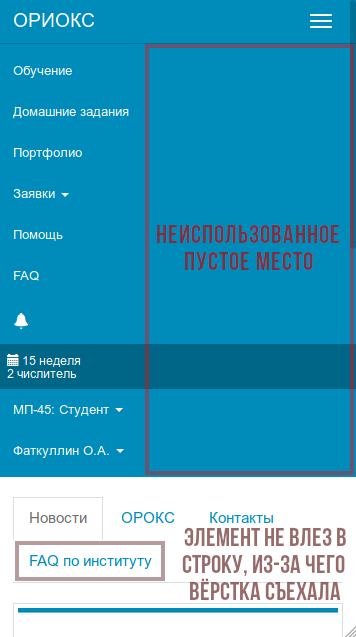
\includegraphics[width=\textwidth/2]{inc/img/orioks_mobile.png}
  \caption{Главная страница ОРИОКС с открытым меню}
  \label{fig:orioksMobile}
\end{figure}

\subsection{Сайт ОРИОКС}
\label{subsec:orioks}

\Define{Платформа}{среда выполнения, в которой должен выполняться фрагмент программного обеспечения или объектный модуль с учётом накладываемых средой ограничений и предоставляемых возможностей}
\Define{Браузер}{программное обеспечение для просмотра информации в сети Интернет}
Платформа: Браузер.

\Abbrev{БД}{база данных}
Из плюсов: cайт ОРИОКС получает информацию напрямую из БД.
Это позволяет позволяет запрашивать только ту информацию, которая нужна в данный момент для отображения страницы.
Можно, так же, отметить наличие всех перечисленных выше возможностей, за исключением просмотра расписания (но его можно посмотреть на сайте МИЭТ)~\cite{orioks}.
Графический интерфейс присутствует, но не полностью адаптирован для мобильных устройств, то есть в некоторых местах элементы интерфейса не помещаются на экране, а в других "--- наоборот слишком много неиспользованного места (см.~рис.~\ref{fig:orioksMobile}).

\Abbrev{HTML}{hypertext markup language "--- язык гипертекстовой разметки}
К минусам можно отнести отсутствие push-уведомлений, невозможность просмотра информации без интернет соединения и необходимость загружать таблицы стилей и HTML разметку для просмотра страницы.

\begin{figure}[ht]
  \centering
  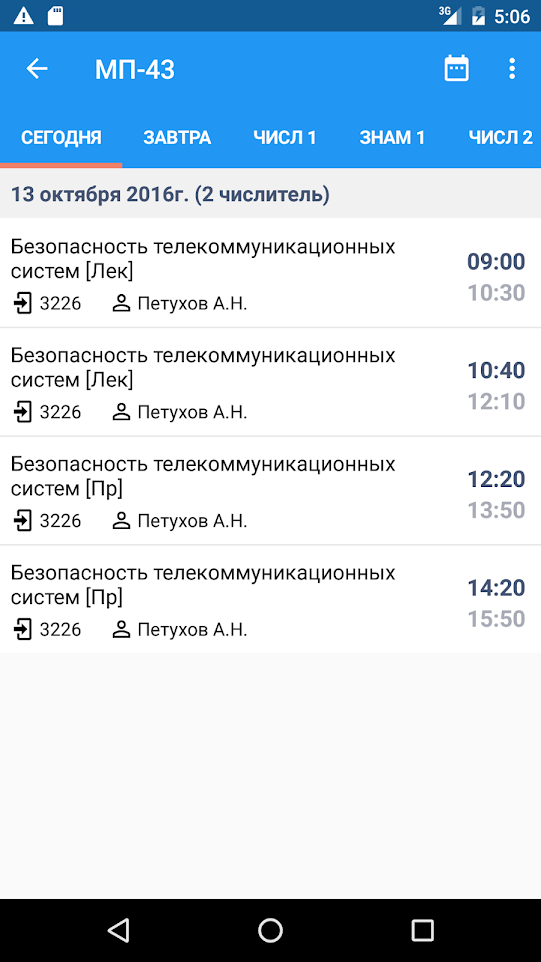
\includegraphics[width=\textwidth/2]{inc/img/miet_schedule.png}
  \caption{Экран расписания в приложении ``Расписание для МИЭТ''}
  \label{fig:mietSchedule}
\end{figure}

\subsection{Приложение ``Расписание для МИЭТ''}
\label{subsec:appMietSchedule}
Платформа: Android.
Дополнительная информация: около тысячи установок;
рейтинг на Google Play "--- 4.7 из 5;
дата последнего обновления "--- 22.04.2018.

Приложение предназначено для просмотра новостей МИЭТ и расписания любой группы с возможностью скачать его и использовать в оффлайн-режиме.
Раньше присутствовал функционал просмотра успеваемости, но из-за изменений на сайте ОРИОКС этот функционал стал недоступен~\cite{market:mietSchedule}.

Получение расписания реализовано через API, это плюс.
Для получения текущей успеваемости использовался синтаксический анализ сайта.
При таком подходе любое изменение в таблице стилей или HTML разметке сайта приводит к неработоспособности приложения, что и случилось.

Из требуемых возможностей присутствует просмотр и кэширование расписания, это позволяет просматривать его без интернет-соединения
Просмотр текущих предметов, успеваемости, списка долгов и пересдач невозможен.

Графический интерфейс присутствует, но не соответствует требованиям Material Design.
Например, слишком маленькие отступы от краёв экрана (см.~рис.~\ref{fig:mietSchedule}).

\begin{figure}[ht]
  \centering
  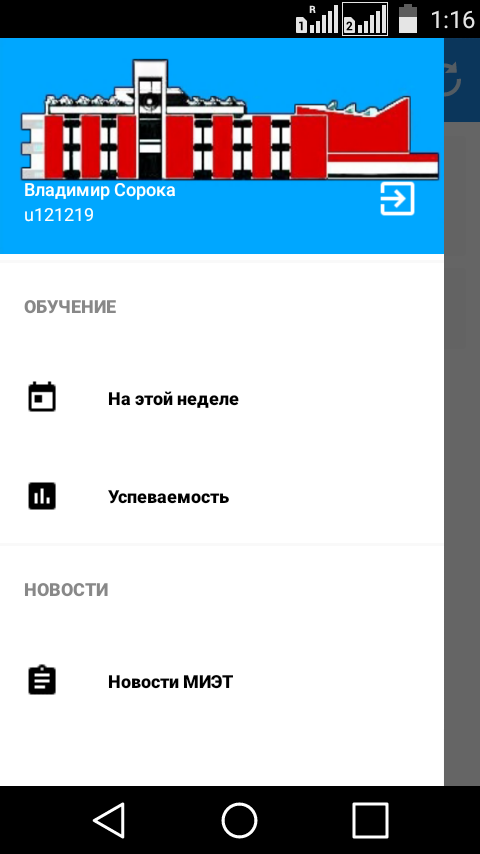
\includegraphics[width=\textwidth/2]{inc/img/orioks_live.png}
  \caption{Главный экран с открытым меню в приложении ``Ориокс Live''}
  \label{fig:orioksLive}
\end{figure}

\subsection{Приложение ``ОРИОКС Live''}
\label{subsec:appOrioksLive}
Платформа: Android.
Дополнительная информация: около тысячи установок;
рейтинг на Google Play "--- 3.9 из 5;
дата последнего обновления "--- 30.09.2015.

Приложение предназначено для просмотра успеваемости, списка контрольных мероприятий и информации о преподавателях~\cite{market:orioksLive}.

Данные получаются при помощи непубличного программного интерфейса, но интерфейс был удалён, т.к. был сделан неофициально и работа с ОРИОКС стала невозможна.
Приложение не обновлялось с 2015 года и на данный момент не работает.

Заявленный функционал проверить не удалось из-за невозможности авторизации, поэтому все эти возможности отметим как отсутствующие.
Рабочей осталась только возможность просмотра новостей.

Графический интерфейс присутствует, но не соответствует требованиям Material Design.
Неправильные отступы, слишком контрастные цвета (см.~рис.~\ref{fig:orioksLive}).

\begin{figure}[ht]
  \centering
  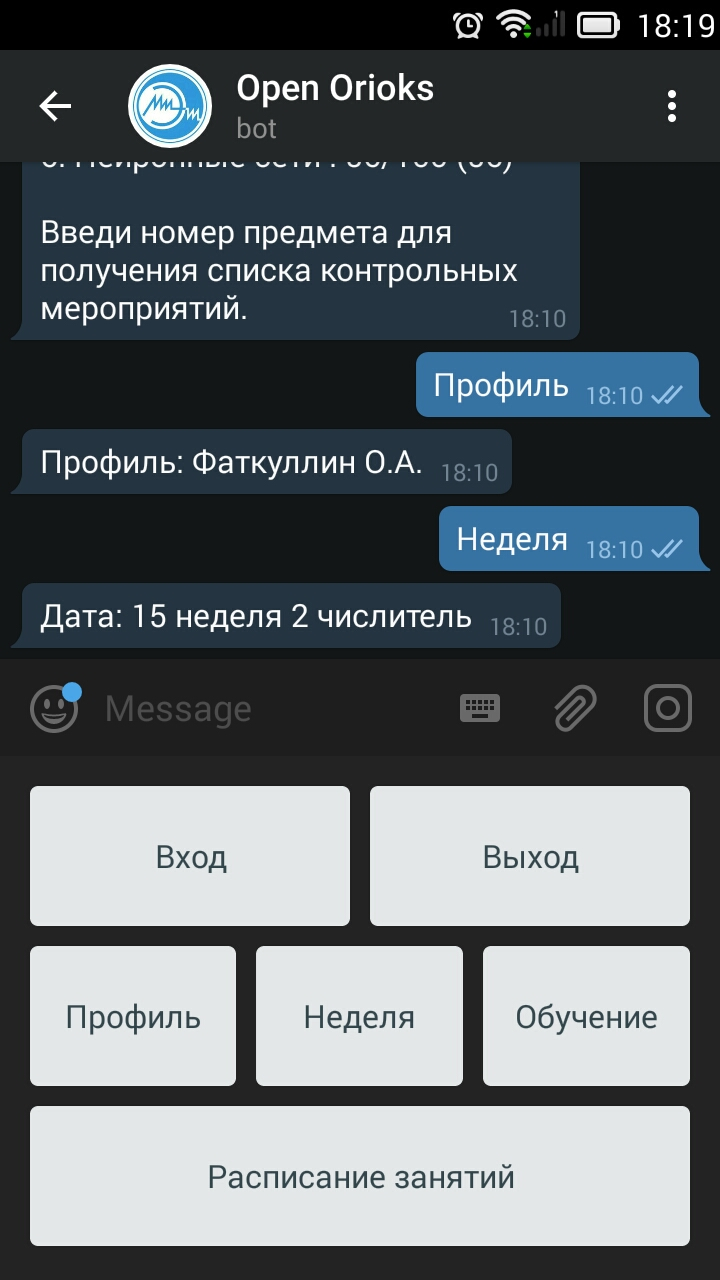
\includegraphics[width=\textwidth/2]{inc/img/open_orioks.jpg}
  \caption{Интерфейс управления Telegram-ботом ``Open Orioks''}
  \label{fig:openOrioks}
\end{figure}

\subsection{Telegram-бот ``Open Orioks''}
\label{subsec:botOpenOrioks}
Платформа: Telegram.
Дополнительная информация: последнее обновление "--- 12.10.2017.

Бот позволяет просматривать расписание на день, текущую успеваемость и список контрольных мероприятий по каждому предмету.

Для получения данных используется синтаксический анализ, но за счёт того, что данные всех студентов обновляются раз в полчаса и сохраняются в хранилище бота, скорость получения данных конечным пользователем сравнима со скоростью получения данных из БД~\cite{github:openOrioks}.

Собственного графического интерфейса нет.
Взаимодействие с ботом производится через текстовые сообщения в мессенджере Telegram.
Использование при отсутствии интернета невозможно, но можно просматривать предыдущие ответы бота, что можно считать частичным кэшированием.

По итогом обзора аналогичных решений была построена таблица~\ref{tab:analogs}.
Как видно из таблицы, нет ни одного решения, которое бы соответствовало всем необходимым параметрам, что еще раз доказывает актуальность задачи.

\begin{table}[ht]
  \caption{Сравнение аналогичных решений}
  \label{tab:analogs}
  \small
  \begin{tabularx}{\textwidth}{|>{\raggedright}m{.203\textwidth}|>{\hsize=.9\hsize}C|>{\hsize=1.2\hsize}C|C|>{\hsize=.9\hsize}C|c|}
    \hline
    Критерий & Сайт ОРИОКС~\cite{orioks} & Приложение ``Расписание для МИЭТ''~\cite{market:mietSchedule} & Приложение ``ОРИОКС Live''~\cite{market:orioksLive} & Бот ``Open Orioks''~\cite{github:openOrioks} & МП СУПС \\
    \hline
    Скорость получения информации & Средняя & Высокая & Низкая  & Средняя & Высокая \\
    \hline
    Push-уведомления              & $-$     & $-$     & $-$     & $+$     & $+$     \\
    \hline
    Расписание                    & $\pm$   & $+$     & $-$     & $\pm$   & $+$     \\
    \hline
    Текущие предметы              & $+$     & $-$     & $-$     & $+$     & $+$     \\
    \hline
    Успеваемость                  & $+$     & $-$     & $-$     & $+$     & $+$     \\
    \hline
    Долги                         & $+$     & $-$     & $-$     & $-$     & $+$     \\
    \hline
    Пересдачи                     & $+$     & $-$     & $-$     & $-$     & $+$     \\
    \hline
    Графический интерфейс         & $+$     & $-$     & $-$     & $-$     & $+$     \\
    \hline
    Оффлайн доступ                & $-$     & $+$     & $-$     & $\pm$   & $+$     \\
    \hline
  \end{tabularx}
  \caption*{
    \small
    \raggedright
    $+$ -- указанная возможность присутствует\\
    $\pm$ -- указанная возможность частично присутствует\\
    $-$ -- указанная возможность отсутствует
  }
\end{table}

В приложении ``Расписание для МИЭТ'' есть кэширование, но работает оно только для расписания, так как остальные функции недоступны.
Только Telegram-бот ``Open Orioks'' предоставляет возможность push-уведомлений, но не обладает всеми требуемыми возможностями, т.к.\ при увеличении количества выполняемых задач, бот становится неудобен в использовании.


\section{Обзор мобильных платформ}
\label{sec:platforms}
Смартфоны, в виде, похожем на нынешний, появились в 2007 году, когда Стив Джобс на выставке ``Macworld Conference \& Expo'' показал миру iPhone.
Все существующие телефоны мгновенно стали устаревшими.
Рынок смартфонов был практически пуст и было понятно, что один iPhone c iOS его не покроет.
В Google в это время только думали о выпуске своего телефона, но о смартфоне речи не шло.

\Abbrev{ОС}{операционная система}
За четыре года до этого, в 2003 году, Энди Рубин, Ник Сир, Крис Уайт и Рич Майнер решили создать операционную систему для носимых устройств, которые могли бы подстраиваться под нужды пользователя.
Они основали компанию Android Inc.\ и назвали свою операционную систему Android.
Никто тогда не оценил этот стартап и в 2005 году компания была на грани банкротства, но Энди Рубин смог убедить Google, которая занималась скупкой инновационных проектов, в том, что у Android есть будущее.
Так и оказалось.

В 2007 году Google вспоминает, что они покупали стартап, направленный на разработку операционной системы для переносных устройств.
Команда Android была только рада заняться разработкой ОС, но нужно было найти производителя смартфонов, который был бы готов выпустить на рынок устройство с совершенно новой ОС.
У Nokia уже была своя ОС "--- Symbian.
Motorola в это время была ослеплена успехом Razr и вряд ли обратила бы внимание на Android.
Оставались еще LG и HTC, но LG уже решили развивать Windows Mobile вместе с Microsoft, поэтому выбор пал на HTC\@.
HTC была рада сотрудничеству с большой компанией и могла обеспечить быстрый выпуск прототипов устройств.
В 2007--2008 году Google и HTC интенсивно работали над первым смартфоном на базе Android "--- HTC Dream.
22 октября 2008 года устройство уже поступило в продажу.

\todo{Добавить инфографику с историей развития мобильных платформ.}

В 2009 году Microsoft тоже попыталась выйти на рынок смартфонов и выпустила Windows Phone 7.
Проект оказался неудачным, своего рода ``мобильная Vista''.
Продажи устройств на Windows Mobile и Symbian упали и остались только две развивающиеся ОС "--- Android и iOS\@.
Apple не позволяла сторонним компаниям использовать iOS, поэтому все взгляды обратились  на Android.

\begin{figure}[ht]
  \centering
  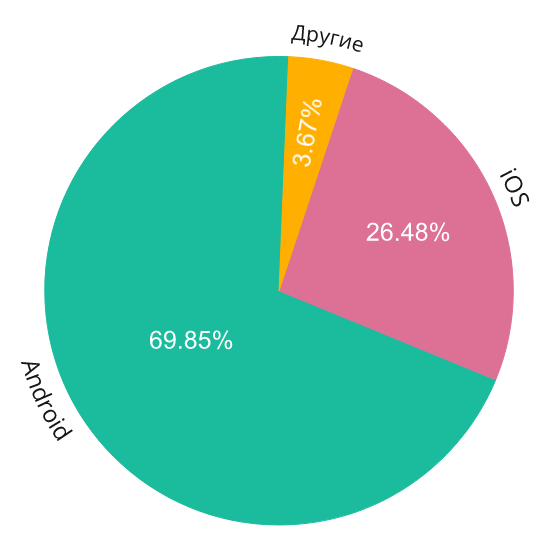
\includegraphics[width=\textwidth/2]{inc/svg/os_popularity}
  \caption{Доля устройств (данные по России)}
  \label{fig:osPopularity}
\end{figure}

Гонка Apple и Google продолжалась.
Компании улучшали свои ОС чтобы превзойти друг друга по быстродействию, безопасности, интерфейсу, функциональности, удобству использования и т.д\@.
В данный момент обе ОС достигли высокого уровня по всем направлениям, но в силу того, что Android "--- открытая система и лицензии (Apache v2 и GNU GPL v2) не запрещают устанавливать адаптировать её под любые устройства, она гораздо популярнее чем iOS\@.

Исходя из доли устройств с каждой мобильной ОС в России (см.~рис.~\ref{fig:osPopularity}), будем выбирать из двух вариантов: iOS и Android.
Разработка для iOS ведется на языке Swift или Objective-C, для работы среды разработки требуется устройство под управлением MacOS~\cite{appleDev}.
Для разработки под Android можно использовать Java или Kotlin, среда разработки не накладывает ограничений на ОС разработчика, так как доступна для Windows, Linux и MacOS~\cite{androidDev}.

\begin{table}[ht]
  \caption{Сравнение мобильных платформ}
  \label{tab:os}
  \begin{tabular*}{\textwidth}{|L|M{0.29\textwidth}|M{0.19\textwidth}|M{0.12\textwidth}|M{0.138\textwidth}|}
    \hline
    Название & Поддерживаемые языки программирования & Доля устройств (Россия)~\cite{statista:os} & Исходный код & ОС для разработки \\
    \hline
    iOS~\cite{appleDev}       & Swift, Objective-C & 26.48\% & Закрытый & MacOS \\
    \hline
    Android~\cite{androidDev} & Kotlin, Java       & 69.85\% & Открытый & GNU\textbackslash Linux, Windows, MacOS \\
    \hline
  \end{tabular*}
\end{table}

Для сравнения была составлена таблица~\ref{tab:os}.
Исходя из покрытия устройств, открытости исходного кода, ограничений на ОС для разработки и наличия опыта программирования на языках Java и Kotlin, была выбрана платформа Android.


\section{Исследование структуры ОРИОКС, концептуальная модель}
\label{sec:orioksStructure}

Функционал ОРИОКС делится на несколько частей, мы будем рассматривать только часть которая касается студентов, и говоря, например, ``инфологическая модель ОРИОКС'' будем иметь ввиду инфологическую модель студенческой части ОРИОКС\@.

На главной странице есть доступ к новостям, FAQ, портфолио, текущей успеваемости.
При открытии страницы успеваемости отображается список предметов, текущий балл по каждому из них и индикатор контрольного мероприятия (если индикатор активен, значит на этой неделе есть контрольное мероприятие по этому предмету).
Список дисциплин одинаков для всех студентов из одной группы.
Но если студент обучается по индивидуально плану, список его предметов будет отличаться.
Кроме того, у каждого студента может быть собственный список долгов, который хранится и отображается отдельно от текущих дисциплин.

Нажатие на строку предмета открывает страницу с подробной информацией, где содержится список преподавателей, форма зачёта, список ресурсов, название кафедры и список контрольных мероприятий.
Для каждого мероприятия выводится:
\begin{itemize}
  \item номер недели когда проходит мероприятие;
  \item название контрольного мероприятия;
  \item форма контроля;
  \item максимальное количество баллов;
  \item текущее количество баллов;
  \item индикатор является контрольное мероприятие обязательным или дополнительным.
\end{itemize}

Расписание не представлено в ОРИОКС, но оно есть на сайте МИЭТ.
Для каждой записи в расписании указывается:
\begin{itemize}
  \item предмет;
  \item день недели;
  \item тип недели (каждую неделю, 1/2 числитель/знаменатель);
  \item номер аудитории;
  \item номер пары;
  \item тип занятия (лабораторная работа, лекция, семинар);
  \item преподаватель.
\end{itemize}

\nocite{db}
\begin{figure}[ht]
  \centering
  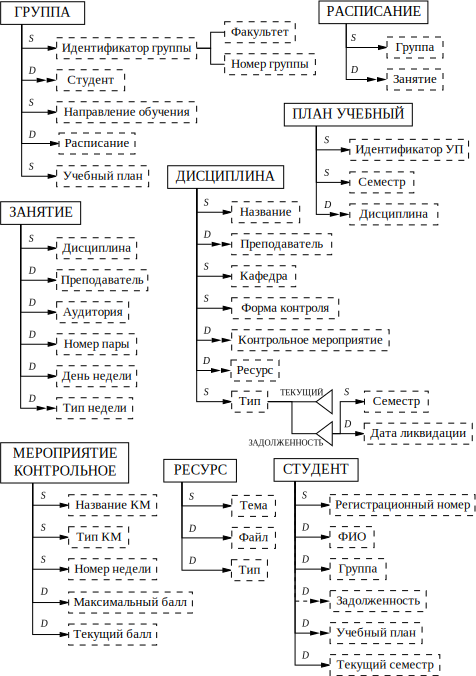
\includegraphics[width=\textwidth]{inc/svg/orioks_concept}
  \caption{Инфологическая модель ОРИОКС}
  \label{fig:orioksConcept}
\end{figure}

\begin{figure}[ht]
  \centering
  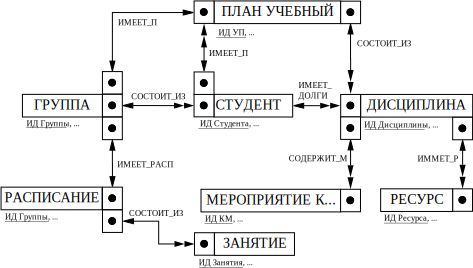
\includegraphics[width=\textwidth]{inc/svg/orioks_er}
  \caption{ER-диаграмма ОРИОКС}
  \label{fig:orioksEr}
\end{figure}

\Abbrev{ИЛМ}{инфологическая модель предметной области}
\Abbrev{ER}{entity-relationship (сущность-связь)}
Можно выделить следующие сущности: группа, студент, план на семестр, ресурс, дисциплина, контрольное мероприятие, расписание, занятие (одна запись из расписания).
Для них была построена ИЛМ (рис.~\ref{fig:orioksConcept}) и ER-диаграмма (рис.~\ref{fig:orioksEr}).


\section{Входные и выходные данные}
\label{sec:io}
В студенческой части ОРИОКС нет полей ввода, кроме формы запроса справки и формы портфолио.
Ввод осуществляется при помощи мыши и заключается в выборе элемента, о котором


\section{Постановка задачи}
\label{sec:problem}

\conclusions
\label{sec:researchConclusions}
